\documentclass[12pt]{article} 
\usepackage{amsmath} 
\usepackage[dvips]{graphicx}
\usepackage{multirow} 
\usepackage{geometry} 
\usepackage{pdflscape}
\usepackage{amsmath}
\usepackage[labelfont=bf]{caption} 
\usepackage{setspace}
\usepackage[running]{lineno} 
% \usepackage[numbers,sort]{natbib}
\usepackage[sort]{natbib} 
\usepackage{array}
\usepackage[table]{xcolor}
\usepackage{xr}
\usepackage{indentfirst}

\newcommand{\methods}{\textit{Materials \& Methods}}
\newcommand{\SI}{\textit{Appendix}~}

\topmargin -1.5cm % 0.0cm 
\oddsidemargin 0.0cm % 0.2cm 
\textwidth 6.5in
\textheight 9.0in % 21cm
\footskip 1.0cm % 1.0cm

\usepackage{authblk}


\title{Species motif participation provides unique information about species risk of extinction}

\author{Alyssa R. Cirtwill$^{1*\dagger}$, Anna \r{A}kesson$^{2*}$, Kate L. Wootton$^{3}$, Anna Ekl\"{o}f$^{2}$} 
\date{
\small$^1$Spatial Foodweb Ecology Group\\
Research Centre for Ecological Change\\
Organismal and Evolutionary Biology Research Programm\\
Faculty of Biological and Environmental Sciences\\
University of Helsinki, Helsinki, Finland\\
\medskip
\small$^2$Department of Theoretical Biology, Chemistry, and Physics\\ 
Link\"{o}ping University, Link\"{o}ping, Sweden\\
\medskip
\small$^3$ BioFrontiers Institute\\
University of Colorado, Boulder, Boulder, U.S.A.\\
\medskip
* Joint first authors\\
\medskip
$^\dagger$ Corresponding author email: alyssa.cirtwill@gmail.com\\
}


\begin{document} 
\maketitle 
\raggedright

\setlength{\parindent}{15pt} 

\section*{Running headline}
Motif participation describes extinction risk

\clearpage

\section*{Summary}


    \indent{1. Bottom-up effects of disturbances to basal resources can strongly affect the persistence of consumers, but it is difficult to predict which species will be most affected by increasing disturbance.} \\
    2. Coarse measures of a species' structural role, like in-degree and trophic level, are known to affect a consumer's vulnerability to bottom-up disturbance. \\
    3. We are interested in whether a richer set of species roles --based on participation in three-species motifs-- is also related to persistence and how these motif-based roles relate to simpler measures. \\
    4. We show that a consumer species' participation in different motifs is related to its probability of persistence. \\ 
    5. Similarly, the overall motif profile of a network is related to the average persistence of consumer species. \\
    6. Notably, we found that networks containing a higher proportion of the `omnivory' motif tend to have lower mean persistence following disturbance, while more frequent participation in the omnivory motif was associated with higher species-level probabilities of persistence. \\
    7. Additionally, we find that relationships between motif participation and persistence can synthesize the information provided by in-degree and trophic level. \\
    8. Motif participation therefore captures important trends in species persistence and provides a rich description of species' structural roles in their communities.


\section*{Key-words}
    food web, degree, trophic level, omnivory, competition

\clearpage
\begin{spacing}{2.0}
\linenumbers

\section*{Introduction} %New

    The loss of a species in a food web can, due to the mutual dependencies among species,  trigger a cascade of additional (secondary) extinctions. 
    A species' position within a food web is known to affect its risk of going secondarily extinct ~\citep{Santos2021,curtsdotter2011robustness, dunne2009cascading, Eklof2006}.
    For example, species with high trophic levels (long paths to basal resources) and low in-degree (few prey) are generally more likely to go extinct~\citep{binzer2011susceptibility, Eklof2006}.
    Species with low in-degree are more vulnerable to extinction because they have few alternative resources if a prey species is lost, while those with high trophic levels are vulnerable to the loss of any species along the path from basal resource(s) to the focal species.
    Based on these trends, it has also been proposed that a species' participation in \emph{meso-scale structures} (which take into account the species' direct and indirect interactions) are also related to its persistence.
    
    
    One way to describe a species' participation in such meso-scale structures is using its participation in the set of \emph{motifs} of a given size~\citep{Cirtwill2015a,Cirtwill2018FoodWebs}.
    Motifs --unique patterns of $n$ interacting species-- correspond to different sets of direct and indirect interactions and provide a holistic description of a species' place in a network~\citep{Stouffer2007,Stouffer2012}.
    Like degree and trophic level, a species' \emph{motif participation} (the vector of frequencies with which it appears in each motif) can easily be calculated once the structure of the network is known.
    However, unlike in-degree and trophic level, which focus only on direct prey of the focal species or on the lengths of paths between the focal species and basal resources, motif participation also incorporates information on the focal species' interaction partners.
    Two species might both have two prey and a trophic level of 3, but they might have quite different motif participation if one species's prey are strict specialists and the others' prey are generalists.
    Importantly, since specialists are generally more vulnerable to extinction than generalists, the predator of specialists will be more likely to lose prey and go extinct itself than will a predator of generalists.
    Therefore, a species' motif participation profile captures the indirect interactions that affect the species, thereby capturing important structures that are missed by larger- or smaller-scale descriptions of the network.
    As such, motif participation may complement degree and trophic level to more fully predict species' extinction risk.
    
    
    The plant community is the foundation upon which the myriad species in food webs depend for their survival. 
    Disturbances to the plant community have been shown to affect important ecosystem properties such as primary \citep{Hector1999} and secondary production \citep{borer2012plant}, soil respiration and carbon cycling \citep{chen2019plant}, and consumer diversity \citep{scherber2010bottom, Baiser2016,li2020bottom}.
    The loss of  basal level diversity typically causes declines in both abundance and richness of all types of consumers: herbivores, predators, parasitoids, etc. \citep{scherber2010bottom,Dobson2009food, Mduma1999food, Georgiadis2007}. 
    Given these far-reaching effects we here choose to analyse persistence after loss of basal resources, i.e., effects of bottom-up disturbances. 
    We are particularly interested in whether the strength of this disturbance affects which consumers are most likely to go extinct. 
    For example, participation in one motif might be associated with greater probability of extinction after a mild disturbance but be associated with less risk of extinction when when more basal resources are lost if the direct and indirect interactions within the motif amplify the effect of small disturbances but also provide the species with alternatives when disturbances are strong.

    
    % While a relationship between motif participation and persistence is broadly intuitive, so far there has been little research demonstrating which motifs are associated with greater probabilities of persistence.
    % One potential reason for the difficulty in assessing the relationship between species' motif roles and persistence are the large computational resources required to simulate population dynamics.
    % Our solution is to use Bayesian networks, which are much more computationally efficient and facilitate the analysis of larger networks~\citep{Eklof2013,Haussler2020}.
    % One limitation with Bayesian networks is that they only take into account bottom-up effects (see Methods). 
    % Nevertheless, Bayesian networks do capture the vast majority of secondary extinctions obtained from fully-fledged dynamical models including top-down and bottom-up effects~\citep{Eklof2013}, and as such are a good proxy for analysing species persistence following extinctions of primary producers in complex food webs.
    % %The greater computational efficiency and similar [[results? performance? extinctions?]] of Bayesian networks allow us to simulate the effects of a gradient of disturbance strength and thereby explore whether participation in some motifs is associated with greater probability of extinction under strong or weak disturbances.

    %There are 13 possible three-species motifs (the most commonly-used size for food web analyses)~\citep{Milo2004,Stouffer2007,Stouffer2012,Cirtwill2015a}, 
    We define motif participation using three-species motifs, which are the most commonly-used size for food web analyses)~\citep{Milo2004,Stouffer2007,Stouffer2012,Cirtwill2015a}. 
    Four of these motifs, namely the three-species chain, apparent competition, direct competition, and omnivory, are especially interesting as they are by far the most common in empirical networks~\citep{Stouffer2007, Borrelli2015a, giling2019plant}.
    These four motifs also have clear ecological interpretations.
    The three-species chain indicates vertical flows of energy and biomass in a network and captures the possibility of indirect interactions across multiple trophic levels (e.g., between a plant and a predator of the plant's herbivore).
    The direct competition motif, where two consumers share the same resource, captures the possibility of indirect interactions between consumers (e.g., by depletion of the shared resource). 
    The apparent competition motif, where a predator consumes two resources, can include indirect effects between prey (e.g., by boosting predator populations) in a top-down context, but in a bottom-up context only includes direct interactions.
    Finally, the omnivory motif, where a predator consumes the same resource as its prey, includes captures the potential for a plant to have both direct and indirect effects on the predator. 
    % Furthermore, these four motifs do not include cycles (where species A and B eat each other or where A eats B eats C eats A).
    % As modelling secondary extinctions using Bayesian networks requires acyclic networks (see Methods), these are the only motifs possible.
    
    
    %\subsection*{Here we test...}
    Here, we analyse whether a consumer's risk of secondary extinction after removal of basal resources depends on the consumer's motif participation and how this relationship varies with the severity of disturbance.
    To provide context for these results, we also consider how a consumer's risk of secondary extinction varies with the overall structure of the network, described by the frequency of motifs across the whole network, network size, and network connectance.
    Finally, we relate species' motif participation to overall network structure and to their in-degrees and trophic levels in order to clarify what unique information motif participation can provide.


    
     %They are also the only motifs which do not include cycles (where species A and B eat each other or where A eats B eats C eats A).
    %As modelling bottom-up extinctions in a Bayesian framework requires the breaking of cycles, these are the only motifs that will appear in the resulting \emph{acyclic} networks.
    %Fortunately, \cite{Allesina2009functional} proved that cyclic and acyclic versions of a network have the same properties in terms of secondary extinctions and the effect on network robustness are very limited. 


%     %\subsection*{1 Why are bottom-up effects important for understanding stability?}
%      The plant community is the foundation upon which the myriad species in food webs depend for their survival.
%      Disturbances to the plant community have been shown to affect important ecosystem properties such as primary \citep{Hector1999} and secondary production \citep{borer2012plant}, soil respiration and carbon cycling \citep{chen2019plant} and consumer diversity \citep{scherber2010bottom, Baiser2016}.
%      As such, the structure of the plant community affects stability across all levels of ecosystem organization, which is crucial for sustaining a healthy energy flow in the ecosystem as a whole~\citep{proulx2010diversity, scherber2010bottom, Rosenblatt2016}. 
%      For example, the loss of diversity at the basal level typically causes declines in both abundance and richness of all types of consumers: herbivores, predators, parasitoids, etc. \citep{scherber2010bottom}.


%     %\subsection*{2 Global and local network properties are known to affect stability}
%     How disturbances such as population decline or extinction lead to the loss of species via direct and indirect effects (i.e., secondary extinctions) has long been a vibrant area of research \citep{Santos2021,curtsdotter2011robustness, dunne2009cascading, Eklof2006}.
%     Several global (whole-network) as well as local (single-species) properties are known to influence how species respond to disturbances. Two well-known, influential global properties are network size, the number of species present in the network, and network connectance, the number of realized feeding interactions.
%     Based on simulations of random networks, large networks were initially thought to be less stable~\citep{May1972}.
%     The indisputable presence of large, persistent empirical networks has spurred research into how other structural characteristics, including connectance, may allow large numbers of species to persist~\citep{Dunne2002}.
%     Highly-connected networks may be more resistant to secondary extinctions because consumers, on average, have access to a larger number of prey species and can switch from a declining or extinct prey to another resource~\citep{Dunne2002, Eklof2006,Baumgartner2015}. However, a well-connected network also includes more pathways through which a disturbance can spread~\citep{Dunne2004, Vieira2015}. Depending on the strength and arrangements of interactions, this means that species may be impacted through several paths, amplifying the original disturbance and causing more secondary extinctions.
%     The net effect of connectance on extinction therefore likely depends on finer-scale (species-level) network structure, as well as the type and severity of disturbance.
    
    
%     Species-level properties known to affect species' responses to disturbances include trophic level (a measure of the path length between a consumer and a basal resource) and in-degree (number of prey items of a predator). 
%     These can also be referred to as local properties of the network.
%     Species with high trophic levels (long paths to basal resources) and low in-degree (few prey) are generally at higher risks of secondary extinction \citep{binzer2011susceptibility, Eklof2006}, and disturbances to plant populations cause particularly many secondary extinctions \citep{Curtsdotter2011}. 
%     However, in-degree and trophic level are both relatively coarse descriptions of a species' role in its food web~\citep{Cirtwill2018FoodWebs}. 
%     A more detailed perspective is desirable since, as well as the properties of the consumer itself, a consumer's risk of secondary extinction after a disturbance to plants depends on the extinction risk of its prey.
%     For example, a generalist consuming many specialist (and therefore high-risk) prey may be at greater risk of extinction than a specialist which consumes a highly generalist resource that is less likely to go extinct (Fig.~\ref{fig:concept}).


%     %\subsection*{3 Motif participation may similarly affect species' particular extinction risk}
%     It is possible to capture information about how a consumer and its prey fit together within a community by defining participation in different motifs -- unique combinations of small numbers of interacting species~\citep{Stouffer2007,Stouffer2012}. 
%     Such motif profiles of species are easily calculated once we know the network structure and require no more information than is used to calculate degree or trophic level.
%     These `motif participation' roles capture information about species' direct as well as indirect interactions, incorporating larger-scale network structure into species-level descriptions~\citep{Cirtwill2015a,Cirtwill2018FoodWebs}.
%     We refer to these motifs as meso-scale structures to emphasise their role as structures between global (network-level) and local (species-level) properties.  
%     A species' motif participation profile shows the second-step indirect interactions the species are affected by, thereby capturing important structures that are missed by global and local properties.  
%     Therefore, by allowing researchers to distinguish between, for example, consumers of specialists and generalists, motif participation may complement degree and trophic level to more fully predict species' extinction risk.
    

%     While the potential relationships between motif participation and species-level extinction risk have not yet been tested to our knowledge, it has been shown that the frequencies of different motifs within a whole network are associated with community stability \citep{prill2005dynamic, bascompte2005simple} and with changes to the composition of plant communities \citep{giling2019plant}. 
%     These relationships between network-level motif frequencies (`motif profiles') and overall community stability mean that a network's motif profile could affect the average extinction risk for consumers within the network.
%     Moreover, if network motif profiles are related to average extinction risk, it is worth investigating whether a species' participation in different motifs also affects its extinction risk.

% % Severity of disturbance
%     As mentioned above, the severity of a disturbance may interact with network structure to affect secondary extinctions.
%     A mild disturbance (e.g., leading to a small increase in the probability of basal resources going extinct) is intuitively likely to cause fewer secondary extinctions than a severe disturbance, and the difference in effects can depend on network structure~\citep{Baumgartner2015}.
%     Empirical studies have shown that disturbances to plant species can affect some consumers more strongly than others \citep{byrnes2011climate}, that the strength of disturbance affects which consumer species are most strongly affected~\citep{detmer2021variation,carnell2020more}, and that the resilience and return time of the ecological community can be strongly influenced by disturbance severity \citep{rydgren2004disturbance}. 
%     The severity of disturbance therefore clearly has an effect on how the ecological community will respond. 

    



\section*{Methods}

    \subsection*{Network construction and describing species roles}

        We generated simulated networks using the niche model, which has been shown to recreate the structure of empirical networks well~\citep{Williams2000,Stouffer2007}.
        To capture a range of network architectures similar to those in well-studied empirical networks~\citep{Dunne2002,Dunne2002e}, we simulated networks with sizes (S) ranging from 50 to 100 species (in steps of 10) and connectances (C) ranging from 0.02 to 0.18 (in steps of 0.04). 
        All networks were generated using the function ``nichemodel'' within the Julia~\citep{Bezanson2017julia} package \emph{BioEnergeticFoodWebs}~\citep{bioenergfw,Delmas2017}.   
        For full details and a comparison to empirical networks, see \emph{Appendix S2}.
        We removed any biologically unlikely networks (i.e., those with extremely long paths between any consumer and basal resources; \emph{Appendix S2}) and replaced them with new simulated networks, repeating the process until we obtained 100 suitable networks in each combination of size and connectance.

        
        % To make the simulated networks compatible with the Bayesian simulation framework, all networks were rendered acyclic following~\citet{Allesina2009functional} and species topologically sorted from lowest to highest trophic level (\emph{Appendix S2}). 
        %  These processing steps allow the strictly bottom-up calculation of probability of persistence.
        We then described each consumer species' motif participation role in each of these simulated networks before applying any disturbance. 
        A species' ``motif participation role'' is the frequency with which the species appears in each of the motifs present in a network~\citep{Stouffer2012}.
        As only four unique three-species motifs can appear in acyclic networks, these are four-dimensional vectors. 
        Here we are interested in the relative frequencies of each motif rather than the total number of motifs and therefore normalized participation vectors by dividing each count by the total number of motifs the species appears in (such that the vector for each species sums to 1).
        Note, however, that this normalization does not necessarily control for differences due to degree or connectance~\citep{Cirtwill2022Oikos}. 


        We also calculated two simpler measures of a species' role within its community.
        In-degree is a species' number of prey.
        Trophic level (shortest trophic level; STL) is the length of the shortest food chain between the focal species and any basal resource~\citep{Williams2004}).
        Both simple role measures were calculated in R~\citep{R} using the same algorithm as~\citet{Eklof2013}.

        
        Finally, to provide context for species' motif participation, we also calculated network ``motif profiles'': four-dimensional vectors of the number of each three-species motif in each network~\citep{Stouffer2012}.
        Together with network size and connectance, these motif profiles describe the structure of the whole network rather than how a particular species participates in the community.
        To separate differences in motif structure from differences in network size or connectance (larger and more-connected networks contain more motifs), we normalized motif profiles by dividing the count of each motif by the total count of all motifs. 
        We calculated species' motif participation using the Python package \emph{pymfinder}~\citep{pymfinder}.



    
    
    \subsection*{Modelling secondary extinction using Bayesian networks}


        Traditionally, there are two main approaches for studying secondary extinctions (i.e., extinctions of species that were not directly disturbed). 
        First, there are topological models, based only on food web structure \citep{dunne2009cascading}. 
        Here, extinctions only affect other species in the network once a consumer has lost all of its prey and therefore must go extinct. 
        The second approach uses dynamical models which explicitly simulate population dynamics using a system of differential equations \citep{binzer2011susceptibility}. 
        Dynamical models take changes in prey or predator densities into account when calculating the densities of other species in the network. 
        This additional detail means that realistic processes such as indirect interactions can be included, but also means that dynamical models are highly parameter intensive and simulations are much more time-consuming than topological models. 
        
        
        A middle‐ground approach for simulating secondary extinctions is to use Bayesian networks, which are much more computationally efficient and facilitate the analysis of larger networks than is practical for dynamical models \citep{Eklof2013,Haussler2020}. 
        In this framework, a consumer's probability of extinction depends on the fraction of resources lost ($f = k/n$ for a species with $n$ resources, of which $k$ have gone extinct) and on a baseline probability of extinction ($\pi$) which captures factors affecting the focal species' extinction probability that are not related to the network structure (e.g., disease, stochastic extinction of small populations).
        Importantly, the greater speed of the Bayesian network framework allows us to simulate a range of disturbance severities rather than single species removals as in many previous studies (e.g.,~\citealp[]{Memmott2004,Staniczenko2010,Dunne2004,Cirtwill2022Oikos}).
        Moreover, Bayesian network simulations are less parameter-intensive than dynamical models, meaning that they are less sensitive to assumptions made in the modelling process~\citep{Eklof2013}.

        % Mention acyclic resstriction here.
        One limitation to Bayesian networks is that consumers do not affect the extinction probabilities of their resources (i.e., only bottom-up effects are included).
        Nevertheless, Bayesian networks do capture the vast majority of secondary extinctions obtained from fully-fledged dynamical models including top-down and bottom-up effects~\citep{Eklof2013}, and as such are a good proxy for analysing species persistence following extinctions of primary producers in complex food webs.
        As our focus in this study is on bottom-up effects from disturbance of basal resources, Bayesian networks will capture the secondary extinctions we are interested in.

        
        Bayesian networks also require the creation of acyclic networks so that a strict bottom-up sequence can be followed. 
        This means that cycles where species A eats species B and vice versa or where A eats B eats C eats A must be broken (see \emph{Appendix SX} for details).
        Since cyclic and acyclic versions of a network have the same properties in terms of secondary extinctions and the effect on network robustness are very limited~\citep{Allesina2009functional}, this change will not strongly affect consumers' extinction risk in our simulations.

        
        The removal of cycles also affects which motifs can appear in the network. 
        Any motif which contains a cycle is impossible in an acyclic network.
        This means that only the four motifs which are most common in empirical networks (\citealp[]{Stouffer2007}: apparent competition, direct competition, omnivory, and the three-species chain) can appear.
        Fortunately, they are also the motifs that have been most studied in isolation (e.g.,~\citep{Hastings1991,Holt1987,Bascompte2005,Polis1989,Zabalo2012,Lefevre2009,Holt1997,Kondoh2008,McKinnon2013,Laws2013}) and have the clearest ecological interpretation and, as such, are of greatest interest to us.


        \subsubsection*{Modelling consumers' risk of secondary extinction}
        
        The response of the consumer to changes in $f$ can take any form (\emph{Appendix S1}). Here we use a sigmoid non-linear function ($\alpha > 1, \beta > 1$), the type of response that most accurately captures the secondary extinctions produced by dynamical models (\citealp[]{Eklof2013}).
		The probability of extinction for each species $i$ can therefore be represented using the cumulative density function of a beta distribution:
		\begin{equation}
		P(\lnot i|f) = \pi + (1 - \pi) \frac{B(f;\alpha,\beta)}{B(\alpha,\beta)}.
				\label{betafunc}
        \end{equation}
		
		If all resource species of a consumer \textit{C} are present ($f = 0$), the extinction probability will be $P(\lnot C|f) = \pi$. 
		Similarly, if all resources are extinct ($f = 1$), the extinction probability $P(\lnot C|f)$ will be equal to 1 and the consumer will go extinct.
		If the fraction $f$ is neither 1 nor 0, the non-linear sigmoid curve will determine the response of the consumer, which will be more severe if the fraction resources lost is high and less severe if the fraction is small. This will in turn affect the extinction probability $P(\lnot C|f)$.
		For basal resources, we assume that abiotic resources are always available and $f=0$. 
		Following Equation \ref{betafunc}, the extinction probability of a basal resource will only depend on $\pi$.
		Note that we here assume that only the fraction, and not the identity, of the resources lost is important. 
		However, the model can easily be modified to incorporate weighted resource interactions \citep[see][]{Eklof2013}.
		
		
		% how we calculate persistences 
        Beginning with basal resources and working systematically up through the food web, we use Equation \ref{betafunc} to calculate each species $i$'s probability of extinction $P(\lnot i|f)$.
        Using this probability, we then perform Bernoulli trials to determine whether the species goes extinct or not. 
        Species are considered extinct if a random number drawn from a uniform distribution $[0-1]$ is less than $P(\lnot i|f)$.
        These simulated extinctions are used when calculating the fraction of resources lost $f$ for each consumer.
        This allows us to update Equation~\ref{betafunc} with information on extinctions of a focal consumer's resources and simulate bottom-up effects. As this method is probabilistic, we repeat these calculations 100 000 times per network, with unique random draws.
        For each species, we then define probability of persistence as the fraction of simulations in which the species persists. 
        While there are methods for solving Bayesian networks exactly \citep{Eklof2013}, for larger networks the numerical evaluation above is highly efficient and produces close to identical results \citep{Haussler2020}.
		
	
		
        \subsubsection*{Disturbance scenarios}
        
            In our un-disturbed scenario, all species had an extinction probability of $\pi = 0.1$. 
            To simulate various threats to basal resources, making some species more vulnerable to extinction, we increase all basal species' probability of extinction from $0.10$ to $0.5$, in steps of $0.08$. 
            The highest disturbance level, $\pi = 0.5$, corresponds to basal species having a 50\% risk of going extinct. 
            Consumer species retained $\pi=0.1$ in all cases.


	\subsection*{Statistical analysis} 
	% Appendix 3, with numbered subheadings.

        We first tested 1) how consumer species persistence varied with motif participation and the severity of disturbance.
        For context, we also test 2) how a consumer's persistence varies with other measures of network structure and a species' place within it.
        As different measures of network structure are not independent since all describe the same network, we also 3) relate species' motif participation to large-scale network structure and to species in-degree and trophic level.
        All analyses are briefly described below and were performed using the R~\citep{R} package \emph{lmerTest}~\citep{lmerTest}.
        % , \emph{MuMIn}~\citep{MuMIn}, and \emph{vegan}~\citep{vegan}.
        See Appendix \emph{3.1 - 3.5} for details. 

        
        \subsubsection*{1) Consumer persistence and motif participation}

            To test whether a consumer's risk of extinction was associated with the frequency of each motif in its participation vector and whether this relationship varied with the strength of disturbance, we fit four general linear models with binomial error distribution (GLMs; one per motif included in the Bayesian networks):
            \begin{equation}
            \Psi_{ink} \approx \rho_{i} + \pi_{k} + \rho_{i}\pi_{k} ,
            % S_{n}C_{n} + N_n,
            \label{propreq}
            \end{equation}
            \noindent where $\Psi_{ink}$ is the persistence of species $i$, belonging to network $n$, during disturbance level $k$, $\rho_{i}$ is the proportion of the role of species $i$ that is made up by the focal motif, and $\pi_k$ is the probability of extinction for a basal resource in disturbance level $k$.
            All predictors were centered and scaled before fitting the models.         

            
            
            Initially, we fit general linear mixed-effect models (GLMMs) also including random  intercepts for the species richness and connectance of network $n$ and for network identity.
            As these models were singular, we removed each random intercept in turn and re-fit the model until it converged.
            In all four cases, the convergent model did not retain any random effects.
            We attempted to fit a PERMANOVA test relating a species' motif participation vector as a whole to its persistence, but the assumption of equal variance among groups was violated and we therefore do not report the results of this test.
            
            
            To test whether these general trends were consistent across networks, we visually examined the distribution of slopes of simplified regressions fit to a single network and level of disturbance.
            These models included only the frequency of the focal motif ($\rho_{i}$ above) and again used a binomial error distrubution.
            To aid in interpretation of these single-network models with respect to network size and connectance, we fit an additional set of GLMs including proportion of motif, strength of disturbance, network size, and connectance across all networks (\emph{Appendix S6}).



        \subsubsection*{2) Consumer persistence and other network structure metrics}

            The overall structure of a network could also affect consumers' ability to persist following a disturbance.
            Here, we describe the overall network structure using the frequency of each motif in the whole network (i.e., the network's motif profile) as well as network size and connectance (which were determined prior to network simulation).
            To test whether the frequency of particular motifs in the network profile were related to the average persistence of all consumers, we fit a set of four GLMs with binomial error distribution (one per motif):
                \begin{equation}
                    \overline{\Psi_{nk}} \approx \Bar{\rho}_{n} + \pi_{k} + \Bar{\rho}_{n}\pi_{k},
                    \label{netpropeq}
                \end{equation}
            \noindent where $\overline{\Psi_{nk}}$ is the mean persistence of all consumers in network $n$ at disturbance level $k$, $\Bar{\rho}_{n}$ is the proportion of the focal motif in the network's motif profile, and $\pi_k$ is the level of disturbance (probability of extinction for basal resources) as in equation~\ref{propreq}.
            As with the GLMs relating each consumer's persistence to its motif participation, we initially attempted to fit GLMMs including random effects of network size and connectance and network identity but removed these random effects in order to obtain non-singular models.


            We also confirmed previously-known relationships between persistence and other measures of network structure or a species' participation in the network.
            To identify the relationship between large-scale network structure and mean probability of persistence within a network, and how the strength of disturbance might affect this relationship, we fit a GLM relating mean persistence to network size, connectance, disturbance, and their interactions.
            As the three-way interaction was significant, we did not simplify the model. 
            

            A consumer's probability of persistence is also known to vary with its in-degree and trophic level.
            To confirm these relationships in our simulated networks and identify how they might vary with different strengths of disturbance, we fit two GLMs with binomial error distribution relating a consumer's persistence to disturbance, in-degree or STL, and the interaction between disturbance and the measure of network participation (\emph{Appendix S3}, Eq. S2-3).
            As with the GLMs relating persistence to motif participation and motif profiles, we initially fit GLMMs including random effects of network size and connectance and network identity but removed these terms due to model singularity.



        \subsubsection*{3) Motif participation and other network structure metrics}

            Since a network's motif profile and a species' motif participation reflect the same network as other measures (size, connectance, degree, and trophic level), it is likely that these measures are related. 
            We tested whether the frequency of motifs in the network's motif profile were related to network size, connectance, and their interaction using a set of four GLMs with binomial error distribution (Appendix \emph{S3}, eq. S4).
            We tested whether the frequency of motifs in a consumer's motif participation vector were related to network size, connectance, and their interaction using a similar set of four GLMs with binomial error distribution.
            Finally, we fit two additional sets of GLMs (eight total) relating the frequency of each motif in a consumer's motif participation vector to the consumer's in-degree or trophic level (Appendix \emph{S3}, Eq. S5-6).
        
        

            
            

            
            




\section*{Results}

    \subsection*{Species persistence and motif participation} 

        A species' probability of persistence was significantly related to its motif participation (Table S1, \emph{Appendix S4}).
        The probability of persistence tended to increase with increasing frequency of the direct competition motif and decrease with increasing frequency of the omnivory motif, across all levels of disturbance.
        The relationships between participation in the apparent competition and three-species chain motifs, however, varied with the strength of disturbance (Fig.~\ref{fig:prop_lmer_all}).
        Higher frequency of participation in the apparent competition motif was associated with lower probability of persistence at low levels of disturbance and higher probability of persistence at high levels of disturbance.
        Participation in the three-species chain motif showed the opposite trends.
    

        In depth exploration of how persistence varied with the proportion of a motif in the species' participation vector, disturbance, and overall network structure (size and connectance), showed that the relationship between the proportion of omnivory in the participation vector and probability of persistence depended strongly on the connectance of the network Fig.~\ref{Fig 2}.
        Higher proportions of omnivory were associated with lower probabilities of persistence when connectance was low, regardless of network size or strength of disturbance.
        At moderate connectance, however, higher proportions of omnivory were associated with greater probabilities of persistence when disturbance was weak.
        In the most-connected networks, higher proportions of omnivory were associated with greater probabilities of persistence at all levels of disturbance.

        The relationships between the proportion of other motifs and persistence were more consistent over different levels of connectance and network size.
        Slopes of the motif proportion-persistence relationships for the apparent competition and direct competition motifs were steepest in large and less-connected networks, but the directions of slopes varied only with the strength of disturbance, as in Fig.~\ref{fig:prop_lmer_all}.
        The relationship between proportion of the three-species chain in the participation vector and persistence was very similar across all levels of size and connectance.
        The effects of network size were overall limited Fig.~\ref{fig:prop_lmer_all}.

        
        Considering each network separately ....
        


    \subsection*{Species persistence and network motif profile}

        As well as the frequency with which each species appears in each motif, we can use the total frequencies of each motif in the whole network (i.e., the network's motif profile) to describe its structure.
        The average probability of persistence of all consumers in the network varied with the frequencies of different motifs in this profile.
        Specifically, average consumer persistence was higher in networks with higher proportions of the apparent competition motif, lower in networks with higher proportions of the omnivory motif, and was not significantly related to the frequencies of the three-species chain or direct competition motifs (Fig. S~\ref{fig:lm_CS}, Table S4, \emph{Appendix S8}). 
        There was no significant interaction between the proportion of any motif in the network profile and level of disturbance (Table S4), \emph{Appendix S8}).


        To provide context for the relationships between consumer persistence and motif participation or motif profile, we also tested whether persistence was related to more commonly used network properties.
        Average consumer persistence was lower in networks with higher connectance, but was not significantly related to network size (Table S6, \emph{Appendix S10}).
        As expected, a consumer's persistence tended to decrease with increasing STL (Fig.~\ref{fig:motifs_vs_TL_and_deg}, Table S3, \emph{Appendix S6}).
        The relationship between in-degree and persistence depended on the strength of disturbance: higher in-degree was associated with greater persistence when basal species had low probability of extinction but lower persistence when basal species were highly likely to go extinct.


    \subsection*{Motif participation and other network properties}

        Both the motif profile of a network and species' motif participation were related to other measures of network structure.
        Most simply, the proportion of the omnivory motif in the network's motif role increased with increasing connectance (Fig. S6, Table S5; \emph{Appendix S9}).
        The proportions of other motifs did not vary significantly with connectance and none were significantly related to network size.


        A species' motif participation varied with network size, connectance, and their interaction. 
        The proportion of the omnivory motif generally increased with increasing connectance and network size, but decreased with increasing network size in the most-connected networks (Fig. S2 and Table S2, \emph{Appendix S5}).
        The proportion of apparent competition decreased strongly with increasing connectance and more weakly (but still significantly) with increasing network size.
        The proportion of the three-species chain showed similar trends to apparent competition, while the proportion of direct competition showed very little change over the range of network size and connectance we consider (though the effects of connectance and the interaction between connectance and network size were significant).

        
        Species' motif participation also varied with their in-degree and trophic level (Fig.~\ref{fig:motifs_vs_TL_and_deg}).
        Species with higher in-degree tended to have higher frequencies of participation in the omnivory motif and lower proportions of the other three motifs.
        Species with higher trophic levels tended to have higher proportions of apparent competition and three-species chains and lower proportions of omnivory and direct competition. 
        A species' persistence varied with both species in-degree and trophic level, where the most clear result is decreased persistence with increased trophic level (Fig.~\ref{fig:motifs_vs_TL_and_deg}; \emph{Appendix S6}). 
        
        
        % \subsubsection*{Consistency in effects of motif participation on species persistence}
    
        %     When fitting regressions of persistence against motif participation for each network separately, networks with high connectance generally showed more consistent relationships between persistence and motif participation, i.e., sharper peaks of the density distributions (Fig.~\ref{fig:density_prop_C}).
        %     However, this trend varied at different levels of disturbance, especially for the direct competition and omnivory motifs.
        %     At low and medium connectances there was little change in the distribution of slopes for direct competition across all levels of disturbance. 
        %     At high connectances, however, the proportion of positive slopes was both lower overall and decreased with increasing disturbance. 
        %     For the omnivory motif these trends were reversed. 
        %     Moreover, the omnivory motif has a particularly broad distribution of slopes (i.e., an inconsistent relationship to persistence) when network connectance was low. 
        %     Network size had a much smaller effect than connectance (Fig. S4; \emph{Appendix S7}).


        




\section*{Discussion}

    The effects of bottom-up disturbances on consumers depend on the large-scale structure of the affected food web~\citep{Dunne2002, Eklof2006, PascualDunne2006}.
    Likewise, the distribution of meso-scale structures within a network affects the network's stability~\citep{prill2005dynamic, bascompte2005simple}.
    In addition, both direct and indirect interactions (i.e., the local and meso-scale structure of a food web  [\citealp[]{Cirtwill2018FoodWebs}]) can affect which species are most strongly affected~\citep{curtsdotter2011robustness, dunne2009cascading, Eklof2006}. 
    Identifying these species is a high priority for conservation efforts~\citep{Bottrilletal2008}.
    To advance this goal, we systematically explore the relationships between meso-scale structures and species' extinction risk, as well as how these trends overlap with the effects of large- and small-scale network properties.

    
    % Species-level results summary
    As with degree and trophic level, a consumer's probability of persistence varied with its participation in different three-species motifs.
    Specifically, increasing participation in the direct competition motif was always associated with higher probability of persistence while increasing participation in the omnivory motif was always associated with lower probability of persistence.
    The relationships between persistence and apparent competition and the three-species chain depended on the strength of the disturbance, with apparent competition associated with greater probability of persistence when basal species were very likely to go extinct and the three-species chain associated with greater probability of persistence at lower levels of disturbance. 
    

    These trends can be partially explained by underlying relationships between motif participation and other measures of a species' place in the network.
    For example, species with higher trophic levels tended to participate less often in the direct competition motif.
    A high trophic level is always associated with lower persistence since predators necessarily have lower probabilities of persistence than their prey~\citep{Eklof2013}.
    Accordingly, high participation in the direct competition motif, by indicating a low trophic level, is associated with high probability of persistence.
    Similarly, participation in apparent competition decreases with increasing in-degree, and probability of persistence shows the opposite trends with respect to in-degree and participation in apparent competition.

    
    The effects of other motifs cannot, however, be attributed so straightforwardly to simpler measures of a species' place in the network.
    Like apparent competition, participation in the three-species chain motif decreases with increasing in-degree, yet persistence varied with the frequency of participation in the three-species chain in the same way as in-degree.
    While participation in the three-species chain motif was positively correlated with trophic level, this cannot explain the relationship between trophic level and probability of persistence as trophic level was negatively correlated with persistence across all levels of disturbance.
    Similarly, higher frequencies of participation in the omnivory motif were associated with lower probabilities of persistence, yet the frequency of the omnivory motif increased with in-degree and decreased with trophic level.
    Both high in-degree and low trophic level are associated with higher probability of persistence, except at high levels of disturbance, which would naively suggest that higher proportions of omnivory should also be associated with greater persistence. 
    Considering a species' in-degree, trophic level, \emph{and} its motif role may therefore provide extra information about its extinction risk.
    
    
    % % Degree and TL are both important for omnivory
    % The relationship between participation in the omnivory motif and persistence connects motif participation with both in-degree and trophic level (STL).
    % Species participation in the omnivory motif was associated with greater persistence, especially at low levels of disturbance.
    % This is consistent with a strong negative correlation between omnivory and trophic level (leading to the overall positive effect of omnivory) and a strong positive correlation with in-degree (leading to the reduced benefit of omnivory at high levels of disturbance). 
    % Motifs can thus act as a tool for synthesizing the information provided by other measures of a species' place in its community and for understanding the interactions among these measures.
    
    
    % % Degree and TL don't explain everything
    % The relationships between persistence and participation in the apparent competition and three-species chain motifs likewise demonstrate the potential for motif participation to synthesize different aspects of network structure.
    % In these cases, in-degree and trophic level are not sufficient to explain the trends we observe in the motifs.
    % For apparent competition, there were strong and opposing correlations with in-degree and trophic level but the relationship between apparent competition and persistence only matches the trends for in-degree.
    % This suggests that some other factor is over-riding the relationship between apparent competition and trophic level.
    
    
    % Similarly, participation in the three-species chain motif was significantly correlated with both in-degree and trophic level, but the relationship between motif participation and persistence did not reflect the disturbance-dependent relationship between in-degree and persistence.
    % This suggests that the relationship between persistence and participation in the chain motif synthesizes the effects of in-degree, trophic level, and some additional effect which counterbalances the effect of in-degree.
    % This additional effect may come from indirect interactions, which are described by motifs but not in-degree~\citep{Cirtwill2018FoodWebs}. 
    
    
    % Moving to network context
    Relationships between a species' probability of persistence and its' position within the network should be considered within the context of overall network structure.
    In our networks, the average probability of persistence of all consumers increased with increasing proportions of the apparent competition, three-species chain, and direct competition motifs and decreased with increasing proportions of the omnivory motif.
    The omnivory motif was also generally less common that the other motifs in these networks, which were selected to be stable before disturbance. 
    
    As well as clarifying the relationships between network structure and the effect of bottom-up disturbance on particular species, motifs were also related to the mean probability of persistence across all species in a network.
    In fact, a network's motif profile had a stronger relationship to mean persistence compared to both network size and connectance. 
    This suggests that network motif profiles may be more useful than large-scale network properties when predicting mean extinction risk of species in a network.
    Connectance did, however, affect which motifs were most common within a network and therefore cannot be entirely ignored. 
    Highly-connected networks tended to contain higher frequencies of the omnivory motif, which includes more links than the other three-species motifs considered here.
    Large-scale properties may therefore indirectly affect network persistence by changing meso-scale properties, such as the distribution of motifs. 
    
    
    In general, average persistence was highest in networks with low proportions of the omnivory motif and high proportions of the apparent competition motif. 
    These results contrast with earlier work showing that higher numbers of omnivory motifs and lower numbers of apparent competition motifs are associated with greater food-web persistence~\citep{Stouffer2010b}.
    By using counts of motifs rather than proportions,~\citet{Stouffer2010b} may be mixing effects of total numbers of motifs with effects of motif proportions.
    Moreover, the effect of omnivory on stability is known to be highly context-dependent \citep{bascompte2005simple, Monteiro2016,McLeod2021}. 
    The stability of omnivory motifs in isolation depends on the strength of the omnivore-resource interaction~\citep{McLeod2021}, but at the whole-network level interactions with other species can stabilize even intrinsically unstable omnivory \citep{Kratina2012}. 
    This might be why we find different patterns between a network's motif profile (where a high proportion of omnivory indicates lower average network persistence) versus a single species motif participation (where a high proportion of the omnivory motif indicates a higher focal species persistence).
    Thus, the ideal situation appears to be being a highly omnivorous species in a low-omnivory setting. 
    
    % High C webs and omnivory
    Supporting this possibility, species participate more frequently in the omnivory motif in high-connectance networks and the relationship between persistence and participation in the omnivory motif is more strongly positive (Fig.~\ref{fig:density_prop_C}) as in~\citet{McLeod2021}.
    These networks contain many pathways by which a bottom-up disturbance can propagate through the network, leading to stronger effects of disturbance on consumers (Table S6; \emph{Appendix S10}).
    In such a network, it may be especially beneficial for a species to feed on multiple trophic levels and, in a sense, spread its risk of losing prey to bottom-up effects.
    Although species in our model cannot swap prey, the reduced extinction risk for omnivorous species resembles empirical studies showing that adaptive omnivory can increase the permanence of three-species chains~\citep{Fagan1997, Kvrivan2005, AbramsFung2010}.
    
    
    There are limitations to the approach presented here.
    Most importantly, the Bayesian network framework operates on a strict bottom-up principle and therefore cannot include top-down effects in the extinction risk calculations~\citep{Eklof2013}. 
    Here our focus was to analyze the importance of disturbances to the basal resources, in which case the Bayesian network approach captures a majority of the secondary extinctions obtained in a fully-fledged dynamical model with much greater efficiency~\citep{Eklof2013}.
    If top-down effects are important for a particular empirical system, however, our simulations may not be accurate. 
    For example, one recent study using a dynamical model shows that time to extinction for species following disturbance is tightly coupled to the motifs a species participates in, and that adding top-down effects can lead omnivory to be negatively correlated with persistence \citep{Cirtwill2021_inprep}. 
    If top-down effects are not crucial, the Bayesian network approach could be extended by explicitly incorporating information on species traits.
    In empirical webs, species traits are related to both motif participation~\citep{cirtwill2018feeding} and extinction risk~\citep{Brose2017, curtsdotter2011robustness, Cardillo2005, Purvis2000},
    adding an extra dimension of information which we do not consider here.
    
    In summary, our results show that participating in different three-species motifs is related to a species' risk of extinction following a bottom-up disturbance, and that these relationships synthesize information provided by other, simpler measures of species roles.
    Critically, our results also underscore the importance of considering the level of disturbance when identifying which species are most at risk of extinction.
    There were strong interactions between the level of disturbance and the relationships between persistence and multiple measures of species roles (motifs and in-degree).
    These simulated results echo other warnings about `tipping points' where previously beneficial traits can become risky~\citep{Latty2019,Golubski2016,Tylianakis2014}.
    For example, at low levels of disturbance a high degree may be protective since species can compensate if one or a few prey are lost. 
    At high disturbance, however, a high-degree species is likely to be affected by disturbances through many paths and have lower persistence.
    These disturbance effects mean that efforts to define a set of target species for conservation interactions must take the current (and future) level of disturbance the community experiences into account.
    
\section*{Acknowledgements}

    The authors thank Gy\"{o}rgy Barab\'{a}s for excellent discussion of the ideas in this manuscript. A{\AA} is supported by the Swedish Research Council for Sustainable Development Formas (\#2015-01262) granted to AE. ARC is supported by a Finnish Academy postdoctoral research grant (\#332999).

\clearpage    

\section*{Figures}
    

        \begin{figure}[hb!]
        \centering
        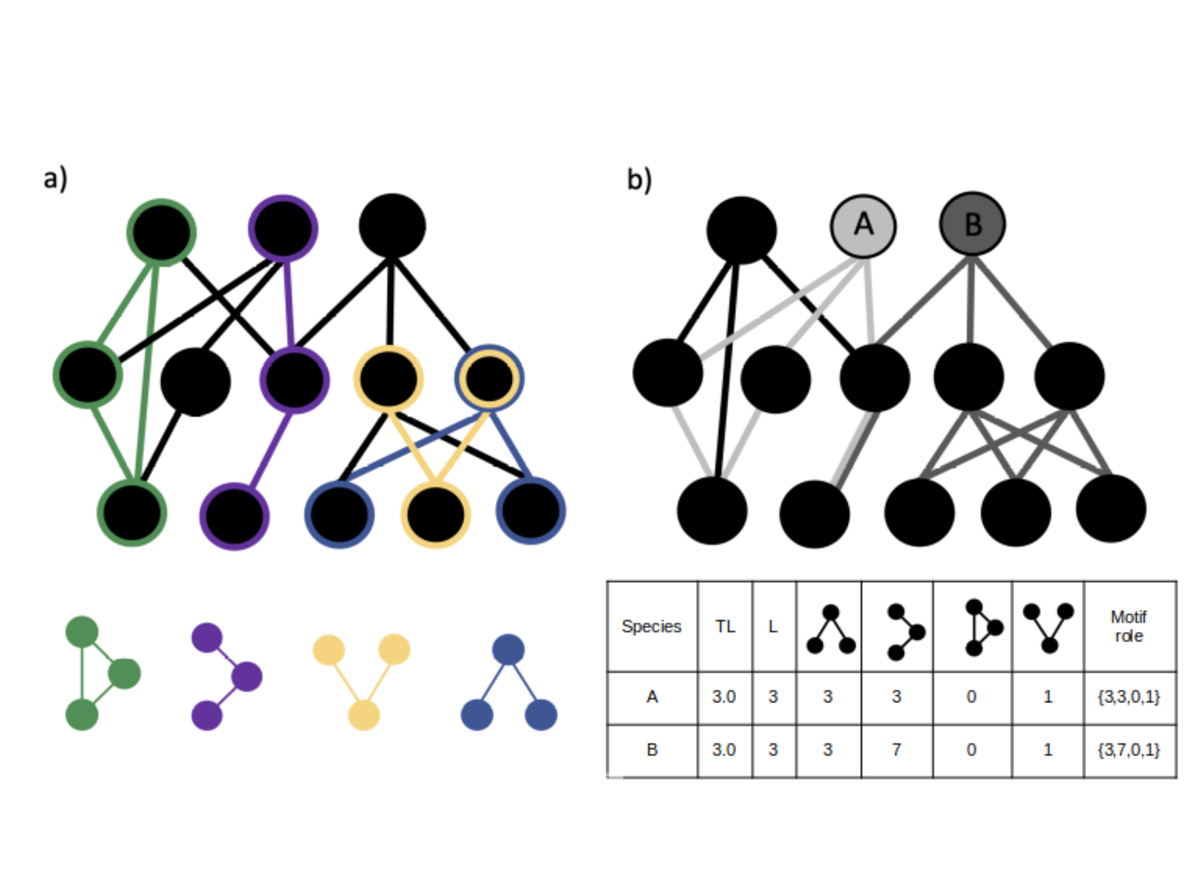
\includegraphics[width=1.0\textwidth]{figures/concept_fig_ver2_edit.eps}
        \caption{Conceptual figure of a toy food web. \textbf{a)} This food web contains examples of the four motifs: apparent competition (blue), three-species chain (purple), omnivory (green), and direct competition (yellow). These motifs capture different ways in which disturbances to basal resources can propagate through the network. For example, a disturbance to the bottom species in a three-species chain will have a direct effect on the middle species but only indirectly affect the top species while a disturbance to the bottom species in an omnivory motif will have a direct effect on the middle species and direct and indirect effects on the top species. 
        Note that the nodes participate in more motifs than the ones highlighted and that a species' motif participation vector is the count of all motifs of each type in which the species appears. \textbf{b)} In the same food web, species with identical degree and trophic level can have different motif participation; here species A (light grey node with links in the same motif colored light grey) participates in only two chains while species B (dark grey node with its direct consumption links colored dark grey) participates in chains more than three times more frequently (see inserted table for counts of participation in all four motifs, giving the motif participation vector in parentheses). 
        Despite having equal degree and trophic level, species A may be at greater risk of going extinct than species B because of its dependence on specialist prey species. Two-thirds of the prey of species B are generalists and therefore more likely to survive a disturbance to basal resources. By including information about indirect interactions, motif profiles reflect this difference between species A and B while trophic level and degree do not.}
    \label{fig:concept}
    \end{figure}

    
        \begin{figure}[hb!]
        \centering
        \includegraphics[width=0.85\textwidth]{figures/persistence_motif_participation.eps}
        \caption{The effect of proportion of the role (x-axis) made up by various motifs (columns) on persistence (y-axis). The effect of participating in each motif is based on the fixed effects in Equation~\ref{propreq}. The different colored lines indicate the probability of extinction of basal species, from $\pi_{disturbed} = 0.1$ (top, purple; no disturbance) to $\pi_{disturbed} = 0.5$ (bottom, yellow; high disturbance). 95\% confidence intervals for each line are shown in grey. Note that omnivory made up a smaller proportion of species' roles than other motifs; lines are plotted over the observed ranges of motif participation.}
    \label{fig:prop_lmer_all}
    \end{figure}
        

    \begin{figure}[hb!]
        \centering
        \includegraphics[width=\textwidth]{figures/roles_vs_TL.eps}
        \caption{Motif participation correlated with in-degree and trophic level, and both of these simpler role measures were also correlated with persistence. \textbf{A)} The proportion of omnivory increased with increasing degree while all other proportions decreased. \textbf{B)} The proportions of omnivory and direct competition decreased with increasing STL while the proportions of apparent competition and three-species chains increased. \textbf{C-F)} The proportion of each motif in consumer's participation vectors varied with connectance, network size, and their interaction (except for apparent competition). We show relationships for the smallest and largest values of network size (S) and connectance (C).
        }
        \label{fig:motifs_vs_TL_and_deg}
    \end{figure}        

    \begin{figure}[ht!]
        \centering
        \includegraphics[width=\textwidth]{figures/persistence_vs_SC_lm.eps}
        \caption{
        \textbf{A} Persistence of consumers increased with increasing in-degree when the probability of extinction for basal resources was low but decreased with increasing in-degree when the probability of extinction was high.
        \textbf{B,E} Mean persistence of consumers in a network decreased strongly with increasing probability of disturbance to basal resources and decreased slightly, but significantly, with increasing connectance. There was no significant relationship between mean persistence and network size.
        \textbf{C} Mean persistence of consumers decreased with increasing proportions of omnivory in the network's motif profile and increased with increasing proportions of other motifs. Persistence also decreased significantly with increasing probability of basal species extinction but there was no significant interaction; we therefore show trends only for $\pi$=0.1.
        \textbf{D} Persistence of consumers decreased with increasing STL at all levels of disturbance.}
        \label{fig:lm_CS}
    \end{figure}


    % \begin{figure}[hb!]
    %     \centering
    %     \includegraphics[width=.9\textwidth]{figures/participation_vs_SC.eps}
    %     \caption{The proportion of each motif in consumer's participation vectors varied with connectance, network size, and their interaction (except for apparent competition). We show relationships for the smallest and largest values of network size (S) and connectance (C).}
    %     \label{fig:roles_vs_SC}
    % \end{figure}


    \begin{figure}[hb!]
    \centering
        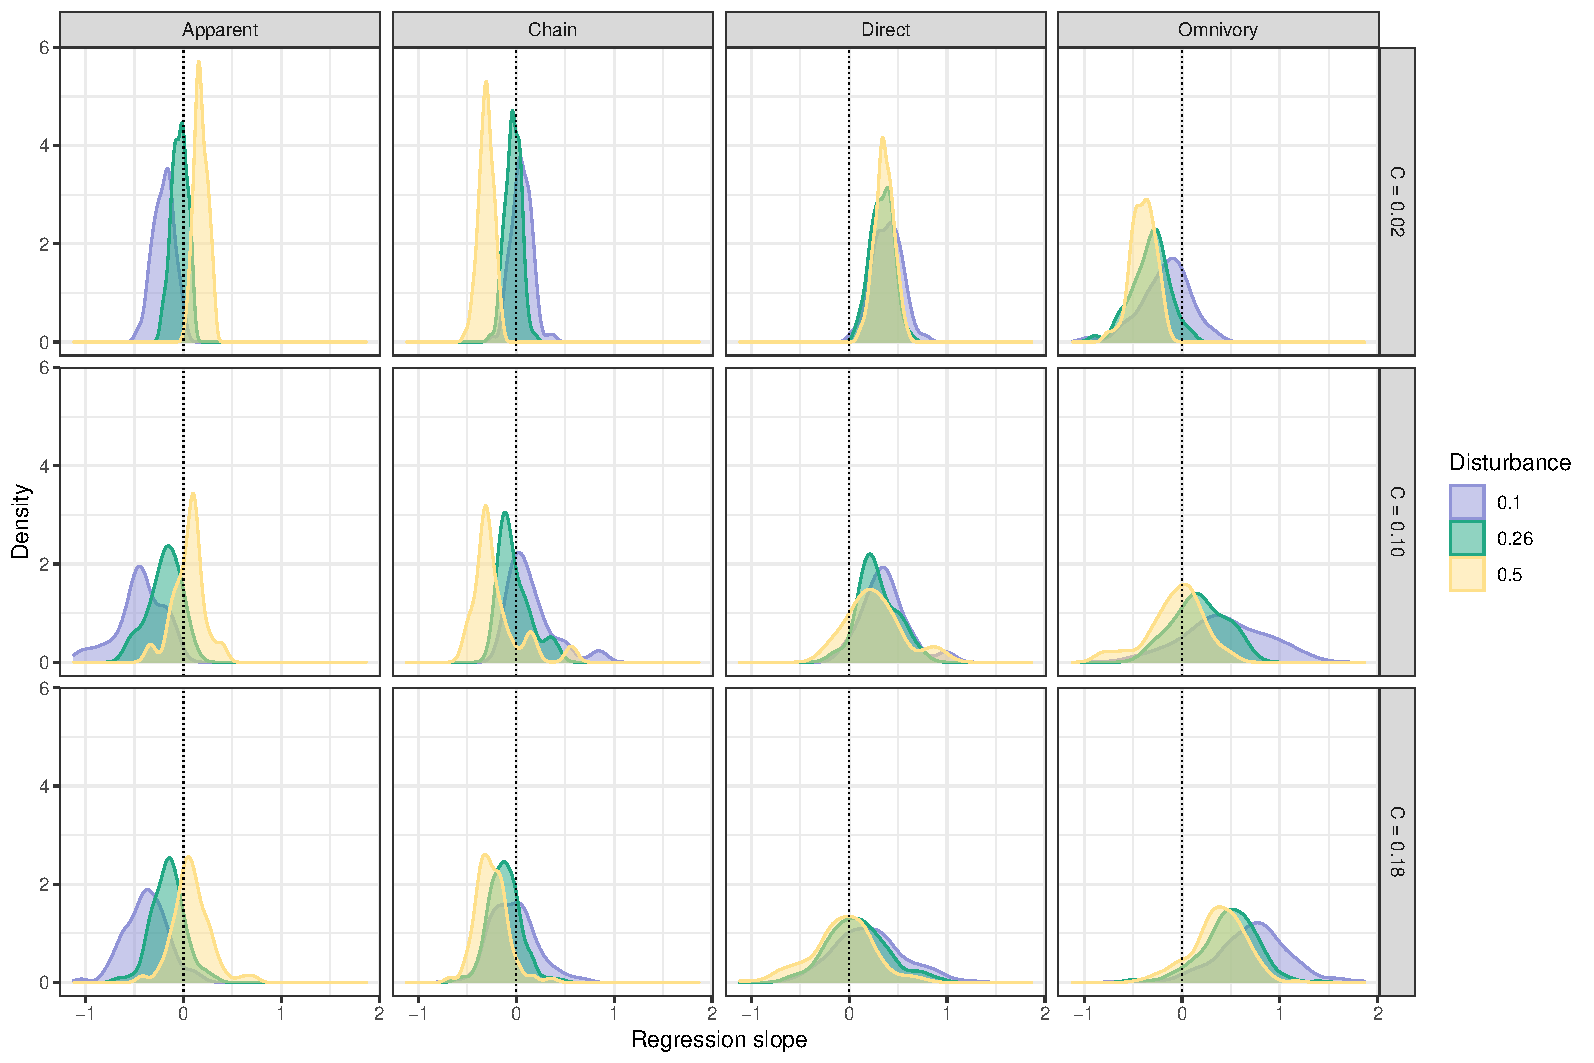
\includegraphics[width=\textwidth]{manuscript/figures/Fig4.pdf}
        \caption{Here we show the density (y-axis) of slopes (x-axis) of persistence against proportion of different motifs for all simulated webs of all sizes - a visualization of how an increased proportion of each motif (different colored lines) affects persistence of consumer species. Columns show the result for various disturbances on the basal level, from $\pi_{disturbed} = 0.1$ (left) to $\pi_{disturbed} = 0.5$ (right). Rows show various levels of connectance. The dotted, vertical lines indicate zero on the x-axis. A negative slope value reflects a negative relationship between increased participation in a motif and persistence, while a positive slope value reflects a positive relationship - an increased proportion of a specific motif increases persistence. The fraction of replicates with a slope greater than zero are stated in numbers in each sub-plot, the color corresponding to each motif (legend). }
        \label{fig:density_prop_C}
    \end{figure}    
    
    % \begin{figure}[hb!]
    %     \centering
    %     \includegraphics[width=\textwidth]{figures/persistence_motif_profiles.eps}
    %     \caption{The proportions of the four motifs in a network's motif profile are related to the mean persistence of species in the network. Specifically, persistence decreases as the proportion of omnivory in the network's motif profile increases while persistence increases with the proportion of the apparent competition motifs. Interactions between motif profiles and disturbance were not significant. Here we show the relationships of probabilities of extinction of basal resources of $\pi=0.1$ (top set of lines) and $\pi=0.5$ (bottom set of lines). Relationships are shown for the observed range of proportions for each motif.}      
    %     \label{fig:motif_profile_persistence}
    % \end{figure}    
    
    % \begin{figure}[hb!]
    %     \centering
    %     \includegraphics[width=\textwidth]{figures/motif_proportion_lms.eps}
    %     \caption{The proportion of the omnivory in a network's motif role increased significantly as connectance increased, while the proportions of the other three motifs did not vary significantly with network size, connectance, or their interaction.}
    %     \label{motif_proportion_lms}
    % \end{figure}




\clearpage

% \section*{Glossary}
% \begin{table}[h!]
% \label{glossary}
% \caption{Glossary of terms relating to motifs and Bayesian networks}
%     \footnotesize{
% \begin{tabular}{l|l}
%     Term & Definition \\
%     \hline
%     Motif & Set of $n$ interacting species. In this case, $n=3$ \\
%     Network motif profile & Vector describing the frequency of each motif in the network. \\
%     & Normalised by dividing counts of each motif by the total across all motifs.\\
%     Motif participation role & Vector describing the frequency with which a focal species appears in each motif.\\
%     & Normalised by dividing counts for each motif by the total across all motifs. \\
%     Bayesian network & A directed acyclic graph, used to predict species' likelihood of persistence. \\
%     Network persistence & The mean likelihood of consumers in a network not going extinct.\\
%     Species persistence & The individual likelihood of a species not going extinct.\\
%     In-degree & Number of prey species to a consumer species.\\
%     Trophic level (STL) & The shortest food chain between the focal species and any basal species.\\
%     Disturbance ($\pi_{disturbed}$) & Probability of extinction of a basal resource when extra disturbance is added. \\
%     Baseline extinction &  When no disturbance is applied, $\pi_{base}$=0.1.\\
% \end{tabular}}
% \end{table}

% Notes on what expressions and words to use
% "probability of extinction" or "level of disturbance" for the different disturbace scenarios?


\bibliographystyle{jae} 
\bibliography{anna_bib_new} % Abbreviate journal titles.

\end{spacing}

\end{document}

